%\VignetteIndexEntry{CGHcall}
%\VignetteDepends{}
%\VignetteKeywords{Calling aberrations for array CGH tumor profiles.}
%\VignettePackage{CGHcall}

\documentclass[11pt]{article}

\usepackage{amsmath}
\usepackage[authoryear,round]{natbib}
\usepackage{hyperref}


\usepackage{/home/mcarlson/arch/x86_64/R-2-7/share/texmf/Sweave}
\begin{document}

\setkeys{Gin}{width=0.99\textwidth}

\title{\bf CGHregions: Dimension reduction for array CGH data with minimal information loss.}

\author{Mark van de Wiel and Sjoerd Vosse}

\maketitle

\begin{center}
Department of Pathology\\
VU University Medical Center
\end{center}

\begin{center}

{\tt mark.vdwiel@vumc.nl}
\end{center}


\tableofcontents

%%%%%%%%%%%%%%%%%%%%%%%%%%%%%%%%%%%%%%%%%%%%%%%%%%%%%%%%%%%%%%%%%%%%%%%%%%%
\section{Overview}

CGHregions allows users to reduce the dimensionality of array CGH data to facilitate downstream analysis. CGHregions takes as input array CGH data (log2-ratios) that have been segmented (i.e., split into chromosomal segments of similar log2-ratios) and called (i.e., a copy number assigned to each segment) on a per-sample basis and adjusts the segmentation so that break-points that are in similar locations across multiple samples are set to be in identical locations. Segmented and called data can be obtained by using the CGHcall package. The resulting dimensionality reduction facilitates downstream analysis in a variety of ways (e.g., reduces severity of multiple hypothesis testing, facilitates clustering and visualization, reduces computer memory requirements). This document provides an overview on the usage of the CGHregions package. For more detailed information on the algorithm and assumptions we refer to the CGHregions article \citep{CGHregions}. As example data we attached the first five samples of the Wilting dataset \citep{Wilting}, called with CGHcall \citep{CGHcall}. 

\section{Example}

In this section we will use CGHregions to define regions of minimal information loss and visualize the results. First, we load the package and the data. The data have been segmented and called using the CGHcall package.

\begin{Schunk}
\begin{Sinput}
> library(CGHregions)
> data(WiltingCalled)
> WiltingCalled
\end{Sinput}
\begin{Soutput}
cghCall (storageMode: lockedEnvironment)
assayData: 3552 features, 5 samples 
  element names: calls, copynumber, probgain, probloss, probnorm, segmented 
phenoData
  sampleNames: AdCA10, SCC27, ..., SCC39  (5 total)
  varLabels and varMetadata description: none
featureData
  featureNames: RP11-465B22, RP4-785P20, ..., CTB-99K24  (3552 total)
  fvarLabels and fvarMetadata description:
    Chromosome: Chromosomal position
    Start: Basepair position start
    End: Basepair position end
experimentData: use 'experimentData(object)'
Annotation:  
\end{Soutput}
\end{Schunk}

\noindent
Next, we apply the {\tt CGHregions} function which returns an object of class cghRegions. For the maximum information loss we allow a value of 0.01.

\begin{Schunk}
\begin{Sinput}
> regions <- CGHregions(WiltingCalled, averror = 0.01)
\end{Sinput}
\begin{Soutput}
                Samples             
 1.00000000  0.00914513 10.00000000 
            Samples           
2.0000000 0.0500994 8.0000000 
[1] "Tuning on small data set finished...started with entire data set"
    Samples     Samples                         
 1.00000000  0.01380531 41.00000000  2.00000000 
Samples Samples         
      0       0      90 
[1] "c = 0, nr of regions: 90"
[1] "Finished with entire data set."
\end{Soutput}
\begin{Sinput}
> regions
\end{Sinput}
\begin{Soutput}
cghRegions (storageMode: lockedEnvironment)
assayData: 90 features, 5 samples 
  element names: regions 
phenoData
  sampleNames: AdCA10, SCC27, ..., SCC39  (5 total)
  varLabels and varMetadata description: none
featureData
  featureNames: 1, 2, ..., 90  (90 total)
  fvarLabels and fvarMetadata description:
    Chromosome: Chromosomal position
    Start: Basepair position start
    ...: ...
    AveDist: Average distance
    (5 total)
experimentData: use 'experimentData(object)'
Annotation:  
\end{Soutput}
\end{Schunk}

\noindent 
As we can see, the algorithm has returned an object with 90 regions. 
To visualize the results we use the {\tt plot} method which creates a plot displaying chromosomes on the Y-axis and base pair position on the X-axis. A new region is displayed by a slight jump with respect to the previous region. Each region is displayed as a bi-colored segment, the lower and upper part of which correspond to the proportions pl and pg of samples with a loss (red) or gain (green), respectively. The color coding is displayed as well: 1: pl (pg) < 10\%; 2: 10\% = pl (pg) < 30\%; 3:30\% = pl (pg) < 50\%; 4: pl (pg) = 50\%.

\begin{center}
\begin{Schunk}
\begin{Sinput}
> plot(regions)
\end{Sinput}
\end{Schunk}
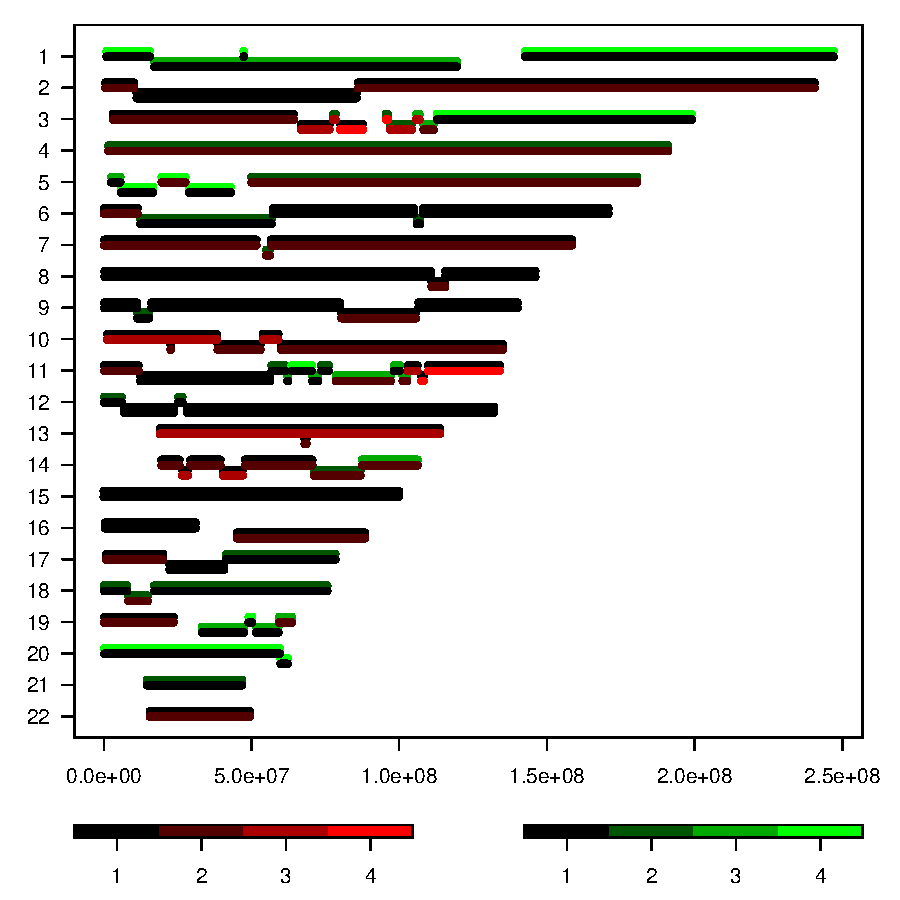
\includegraphics{CGHregions-003}
\end{center}

\pagebreak

\bibliographystyle{apalike}
\bibliography{CGHregions}

\end{document}
